\documentclass[10pt,a4paper]{article}
\usepackage[top=1.5cm, bottom=1.5cm, left=1.6cm, right=1.6cm, headheight=14pt, footskip=18pt]{geometry}
\usepackage[utf8]{inputenc}
\usepackage{amsmath,amsfonts,amssymb}
\usepackage{graphicx}
\usepackage{tikz}
\usepackage{circuitikz}
\usetikzlibrary{calc,patterns}
\usepackage[most]{tcolorbox}
\usepackage{enumitem}
\usepackage{fancyhdr}
\usepackage{booktabs}
\usepackage{tabularx}
\usepackage{colortbl}
\usepackage{hyperref}

% --- Palet Warna Resmi UNIB ---
\definecolor{unibblue}{RGB}{0, 32, 96}
\definecolor{unibgold}{RGB}{197, 160, 89}
\definecolor{unibgreen}{RGB}{34, 112, 60}
\definecolor{boxbg}{RGB}{248, 250, 253}
\definecolor{linegray}{RGB}{210, 215, 225}

% --- Pengaturan Header & Footer ---
\pagestyle{fancy}
\fancyhf{}
\lhead{\footnotesize\textbf{\color{unibblue}Universitas Bengkulu} \textbar\ Program Studi S1 Teknik Elektro}
\rhead{\footnotesize\color{gray}Persamaan Diferensial (Genap 2026)}
\lfoot{\footnotesize\color{gray}LKM OBE \textbar\ \textbf{Video}: \url{https://youtu.be/piBpNjXaKpQ} \textbar\ \href{https://www.youtube.com/playlist?list=PLS5oOZWXZeTw}{\color{unibblue}\textbf{Playlist}}}
\cfoot{\footnotesize\color{gray}Hal. \thepage\ dari 2}
\rfoot{\footnotesize\color{unibblue}\textbf{Minggu 12: Persamaan Panas 1D \& Kemampuan H...}}
\renewcommand{\headrulewidth}{0.6pt}
\renewcommand{\footrulewidth}{0.4pt}

% --- Custom Box untuk Lembar Jawab ---
\newtcolorbox{answerbox}[1]{%
  colback=white,
  colframe=unibblue!70!black,
  coltitle=white,
  fonttitle=\bfseries\scriptsize,
  colbacktitle=unibblue,
  title={#1},
  arc=2pt,
  left=5pt,right=5pt,top=3pt,bottom=3pt,
  boxrule=0.6pt
}

\begin{document}

% ==================== HALAMAN 1 ====================
\noindent\begin{minipage}[c]{0.68\textwidth}%
  {\large\textbf{\color{unibblue}LEMBAR KERJA MAHASISWA (LKM)}}\\[1mm]
  {\normalsize\textbf{Mata Kuliah: Persamaan Diferensial (2 SKS)}}\\[0.5mm]
  {\small\textbf{Topik Minggu 12:} Persamaan Panas 1D \& Kemampuan Hantar Arus Kabel XLPE}%
\end{minipage}%
\hfill%
\begin{minipage}[c]{0.30\textwidth}%
  \begin{tcolorbox}[colback=unibblue!5,colframe=unibblue,boxrule=0.6pt,arc=2pt,left=4pt,right=4pt,top=2pt,bottom=2pt]
    \scriptsize
    \textbf{Nama:} \dotfill\\[1.2mm]
    \textbf{NPM:} \dotfill\\[1.2mm]
    \textbf{Kelas/Klp:} \dotfill\\[1.2mm]
    \textbf{Nilai Final:} \hfill \textbf{/ 100}
  \end{tcolorbox}%
\end{minipage}\par

\vspace{1.5mm}

% Kotak Sub-CPMK & Pedoman
\begin{tcolorbox}[colback=boxbg,colframe=unibgold!90!black,boxrule=0.6pt,arc=2pt,left=5pt,right=5pt,top=3pt,bottom=3pt,title=\textbf{\scriptsize Capaian Pembelajaran (Sub-CPMK 6) \& Pedoman Evaluasi OBE}]
  \scriptsize
  \textbf{Sub-CPMK 6:} Mahasiswa mampu memformulasikan persamaan difusi panas 1D dengan suku pembangkitan kalor Joule serta mengevaluasi batas kemampuan hantar arus kabel tanah sesuai IEC 60287.\\
  \textbf{Video Panduan (YouTube):} \url{https://youtu.be/piBpNjXaKpQ} \hfill \textbf{Playlist:} \href{https://www.youtube.com/playlist?list=PLS5oOZWXZeTw}{\color{unibblue}\textbf{bit.ly/pd-unib-playlist}}\\\textbf{Alokasi Waktu:} 50--60 Menit \quad\textbar\quad \textbf{Model:} Kolaboratif / Mandiri Terstruktur \quad\textbar\quad \textbf{Bahasa Komputasi:} Julia 1.12+
\end{tcolorbox}

\vspace{1mm}

% Soal C1
\noindent\textbf{1. (C1 - Mengingat \textbar\ Bobot: 10 Poin)}\par\vspace{0.5mm}
{\footnotesize Tuliskan bentuk baku Persamaan Panas 1D dengan suku sumber kalor Joule internal: $\frac{\partial u}{\partial t} = \alpha \frac{\partial^2 u}{\partial x^2} + \frac{q_{\text{gen}}}{\rho c_p}$, dan sebutkan definisi fisis konduktivitas termal $k$ serta difusivitas termal $\alpha$.}
\begin{answerbox}{Ruang Pengerjaan C1 (Persamaan Difusi Termal dengan Pembangkitan Kalor)}
  \vspace{2.0cm}
\end{answerbox}

\vspace{1mm}

% Soal C2
\noindent\textbf{2. (C2 - Memahami \textbar\ Bobot: 15 Poin)}\par\vspace{0.5mm}
{\footnotesize Jelaskan metode pemecahan transien termal menggunakan dekomposisi tunak-transien $u(x,t) = u_{\text{ss}}(x) + u_{\text{tr}}(x,t)$. Mengapa solusi tunak $u_{\text{ss}}(x)$ memenuhi persamaan Poisson/Laplace 1D sementara komponen transien meluruh menuju nol?}
\begin{answerbox}{Ruang Pengerjaan C2 (Prinsip Dekomposisi Solusi Tunak dan Transien Kalor)}
  \vspace{2.1cm}
\end{answerbox}

\vspace{1mm}

% Soal C3
\noindent\textbf{3. (C3 - Menerapkan \textbar\ Bobot: 20 Poin)}\par\vspace{0.5mm}
\noindent\begin{minipage}[t]{0.60\textwidth}%
  {\footnotesize Sebuah kabel tanah berisolasi XLPE 20 kV memiliki ketebalan isolasi $d=15\text{ mm}$. Pada kondisi tunak, rugi tembaga menghasilkan fluks panas konstan pada konduktor ($x=0$) sehingga $-k \left.\frac{\partial u}{\partial x}\right|_{x=0} = q_0$, sementara permukaan luar ($x=d$) dijaga pada suhu tanah $T_{\text{tanah}} = 25^\circ\text{C}$. Turunkan profil temperatur tunak $u_{\text{ss}}(x)$.}%
\end{minipage}%
\hfill%
\begin{minipage}[t]{0.37\textwidth}%
  \centering
  \resizebox{0.95\linewidth}{!}{%
  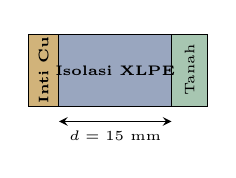
\begin{tikzpicture}[scale=0.65]
    \draw[fill=unibgold!80] (0,0) rectangle (0.6,1.4);
    \draw[fill=unibblue!40] (0.6,0) rectangle (2.8,1.4);
    \draw[fill=unibgreen!40] (2.8,0) rectangle (3.5,1.4);
    \node at (0.3,0.7) [font=\tiny\bfseries, rotate=90] {Inti Cu};
    \node at (1.7,0.7) [font=\tiny\bfseries] {Isolasi XLPE};
    \node at (3.15,0.7) [font=\tiny, rotate=90] {Tanah};
    \draw[<->, >=stealth] (0.6,-0.3) -- (2.8,-0.3) node[midway, below, font=\tiny] {$d=15\text{ mm}$};
  \end{tikzpicture}%
  }%
\end{minipage}\par\vspace{1mm}
\begin{answerbox}{Ruang Pengerjaan C3 (Penurunan Profil Suhu Tunak Isolasi Kabel)}
  \vspace{2.8cm}
\end{answerbox}

\newpage
% ==================== HALAMAN 2 ====================

% Soal C4
\noindent\textbf{4. (C4 - Menganalisis \textbar\ Bobot: 20 Poin)}\par\vspace{0.5mm}
{\footnotesize Analisis Batas Kemampuan Hantar Arus (\textit{Ampacity}) kabel tanah menurut standar \textbf{IEC 60287}: Jika temperatur operasi kontinu maksimum isolasi XLPE tidak boleh melampaui $90^\circ\text{C}$, analisis hubungan antara arus beban maksimum $I_{\text{maks}}$ dengan resistansi konduktor $R_{\text{ac}}$ dan resistansi termal lingkungan $R_{\text{th,total}}$.}
\begin{answerbox}{Ruang Pengerjaan C4 (Analisis Ampacity Kabel Tanah Sesuai Standar IEC 60287)}
  \vspace{3.8cm}
\end{answerbox}

\vspace{1.5mm}

% Soal C5
\noindent\textbf{5. (C5 - Mengevaluasi \textbar\ Bobot: 20 Poin)}\par\vspace{0.5mm}
{\footnotesize Evaluasi risiko *thermal runaway*: Sifat resistansi konduktor meningkat linier terhadap suhu: $R(T) = R_0(1 + \alpha_{\text{Cu}} \Delta T)$. Evaluasi bagaimana umpan balik positif antara kenaikan suhu dan peningkatan disipasi Joule dapat memicu ketidakstabilan termal jika disipasi ke tanah tersumbat.}
\begin{answerbox}{Ruang Pengerjaan C5 (Evaluasi Stabilitas Termal \& Risiko Kegagalan Dielektrik)}
  \vspace{3.8cm}
\end{answerbox}

\vspace{1.5mm}

% Soal C6
\noindent\textbf{6. (C6 - Merancang \& Komputasi Julia \textbar\ Bobot: 15 Poin)}\par\vspace{0.5mm}
{\footnotesize Rancang kode simulasi beda hingga (FDM skema eksplisit FTCS) dalam bahasa \textbf{Julia} untuk menyelesaikan persamaan difusi panas 1D pada batang tembaga. Pastikan kriteria stabilitas numerik Von Neumann $\Delta t \le \frac{\Delta x^2}{2\alpha}$ terpenuhi.}
\begin{answerbox}{Ruang Pengerjaan C6 (Skrip Algoritma FDM Difusi Termal Julia)}
  \vspace{3.8cm}
\end{answerbox}

\vspace{1.5mm}

% Tabel Rekapitulasi Skor OBE & Tanda Tangan
\noindent\begin{minipage}[b]{0.65\textwidth}%
  \centering
  \scriptsize
  \begin{tabular}{|c|c|c|c|c|c|c|}
    \hline
    \rowcolor{unibblue}
    \textbf{\color{white}C1} & \textbf{\color{white}C2} & \textbf{\color{white}C3} & \textbf{\color{white}C4} & \textbf{\color{white}C5} & \textbf{\color{white}C6} & \textbf{\color{white}Total} \\
    \rowcolor{unibblue!10}
    10 Pts & 15 Pts & 20 Pts & 20 Pts & 20 Pts & 15 Pts & 100 Pts \\
    \hline
    & & & & & & \\[2.5mm]
    \hline
  \end{tabular}%
\end{minipage}%
\hfill%
\begin{minipage}[b]{0.32\textwidth}%
  \centering
  \scriptsize
  \textbf{Verifikasi Dosen / Asisten:}\\[5mm]
  (\dotfill)
\end{minipage}\par

\end{document}
